\documentclass[letterpaper]{article}
\usepackage{tikz}
% Set tiny margins so it fits on one sheet
\usepackage[top=10mm,left=5mm]{geometry}
\usetikzlibrary{calendar}
% Get rid of blank page 1
\usepackage{atbegshi}% http://ctan.org/pkg/atbegshi
\AtBeginDocument{\AtBeginShipoutNext{\AtBeginShipoutDiscard}}
\begin{document}
% No page numbers
\pagestyle{empty}
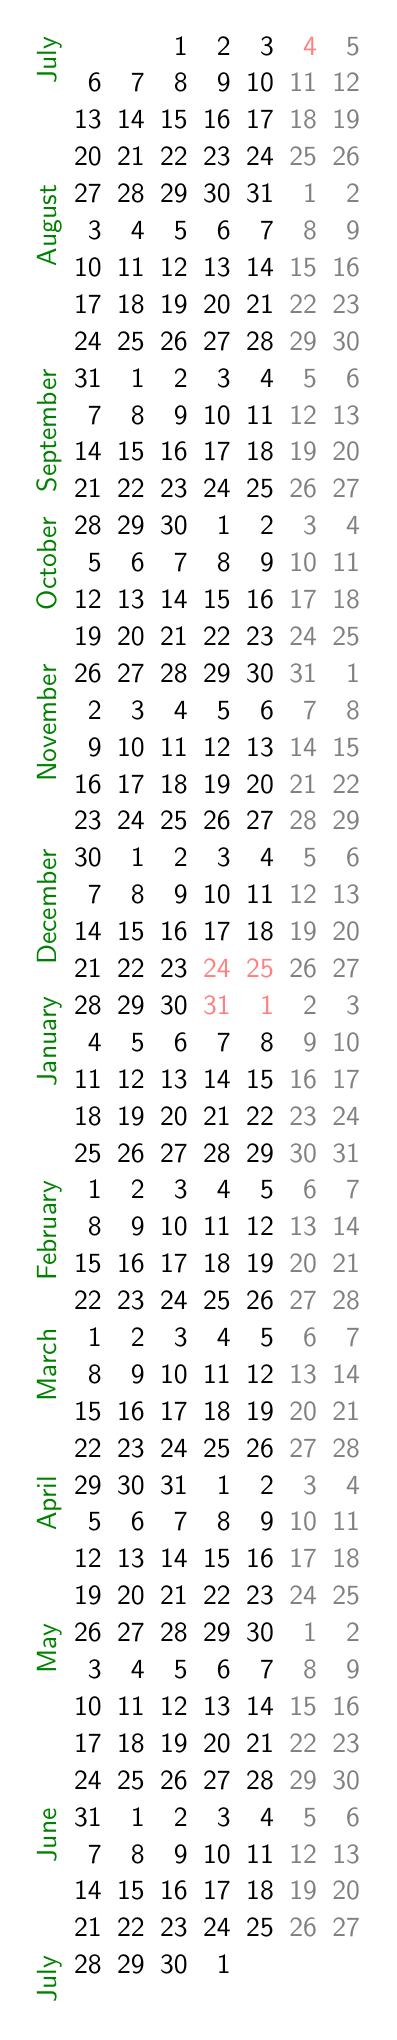
\begin{tikzpicture}
\normalsize\sffamily
% Set colors to 50% throughout so they will work on a black and white printer
\colorlet{darkgreen}{green!50!black}
% Create a running 12 month calendar starting from the current month
\calendar[dates=\year-\month-01 to \year-\month-01+365,week list,
month label left vertical,month yshift=0pt,
month text=\textcolor{darkgreen}{\%mt}]
% Weekends are grey
if (weekend) [black!50]
% Regular holidays are red
if (
    equals=01-01,
    equals=07-04,
    equals=12-24,
    equals=12-25,
    equals=12-31,
   ) [red!50]
% Holidays that vary by year are red
if (
    equals=2024-02-19,
    equals=2024-03-29,
    equals=2024-05-27,
    equals=2024-06-19,
    equals=2024-09-02,
    equals=2024-11-28,
    equals=2025-01-20,
    ) [red!50];
\end{tikzpicture}
\end{document}
